% ser-2017-aha-slcs.Rnw

%---------------------------------------------------------------
% Preamble
% --------------------------------------------------------------
%
% NOTE: See rice-sample.tex written by Daina Chiba at Rice University for formatting and preamble code that I copied, http://ricebeamer.dynaman.net/
\documentclass[final]{beamer}\usepackage[]{graphicx}\usepackage[]{color}
%% maxwidth is the original width if it is less than linewidth
%% otherwise use linewidth (to make sure the graphics do not exceed the margin)
\makeatletter
\def\maxwidth{ %
  \ifdim\Gin@nat@width>\linewidth
    \linewidth
  \else
    \Gin@nat@width
  \fi
}
\makeatother

\definecolor{fgcolor}{rgb}{0.345, 0.345, 0.345}
\newcommand{\hlnum}[1]{\textcolor[rgb]{0.686,0.059,0.569}{#1}}%
\newcommand{\hlstr}[1]{\textcolor[rgb]{0.192,0.494,0.8}{#1}}%
\newcommand{\hlcom}[1]{\textcolor[rgb]{0.678,0.584,0.686}{\textit{#1}}}%
\newcommand{\hlopt}[1]{\textcolor[rgb]{0,0,0}{#1}}%
\newcommand{\hlstd}[1]{\textcolor[rgb]{0.345,0.345,0.345}{#1}}%
\newcommand{\hlkwa}[1]{\textcolor[rgb]{0.161,0.373,0.58}{\textbf{#1}}}%
\newcommand{\hlkwb}[1]{\textcolor[rgb]{0.69,0.353,0.396}{#1}}%
\newcommand{\hlkwc}[1]{\textcolor[rgb]{0.333,0.667,0.333}{#1}}%
\newcommand{\hlkwd}[1]{\textcolor[rgb]{0.737,0.353,0.396}{\textbf{#1}}}%
\let\hlipl\hlkwb

\usepackage{framed}
\makeatletter
\newenvironment{kframe}{%
 \def\at@end@of@kframe{}%
 \ifinner\ifhmode%
  \def\at@end@of@kframe{\end{minipage}}%
  \begin{minipage}{\columnwidth}%
 \fi\fi%
 \def\FrameCommand##1{\hskip\@totalleftmargin \hskip-\fboxsep
 \colorbox{shadecolor}{##1}\hskip-\fboxsep
     % There is no \\@totalrightmargin, so:
     \hskip-\linewidth \hskip-\@totalleftmargin \hskip\columnwidth}%
 \MakeFramed {\advance\hsize-\width
   \@totalleftmargin\z@ \linewidth\hsize
   \@setminipage}}%
 {\par\unskip\endMakeFramed%
 \at@end@of@kframe}
\makeatother

\definecolor{shadecolor}{rgb}{.97, .97, .97}
\definecolor{messagecolor}{rgb}{0, 0, 0}
\definecolor{warningcolor}{rgb}{1, 0, 1}
\definecolor{errorcolor}{rgb}{1, 0, 0}
\newenvironment{knitrout}{}{} % an empty environment to be redefined in TeX

\usepackage{alltt}
\usepackage[orientation=landscape, size=custom, width=121.92, height=106.68, scale=1.7]{beamerposter}  % this matches 4 feet (48 inches) by 3.5 feet (42 inches). Will get from phdposters.com 1 inch per 2.54 cm

\mode<presentation>{\usetheme{UNC5}}
\usepackage[english]{babel}
\usepackage[latin1]{inputenc}
\usepackage{bm}
\usepackage{blindtext}
\usepackage{scrextend}
\addtokomafont{labelinglabel}{\sffamily}
\usepackage{csquotes}
\usepackage{booktabs}

\setbeamercolor{bibliography entry title}{fg=black,bg=black}% see http://tex.stackexchange.com/questions/71352/beamer-undefined-color-local-structure
\setbeamertemplate{caption}[numbered]

% got from http://tex.stackexchange.com/questions/48023/mimic-bibtex-apalike-with-biblatex-biblatex-apa-broken
\PassOptionsToPackage{
        style=numeric,
        hyperref=true,
        backend=bibtex,
        maxbibnames=1,
        firstinits=true,
        uniquename=init,
        maxcitenames=2,
        parentracker=true,
        url=false,
        doi=true,
        isbn=false,
        eprint=false,
        backref=false,
            }{biblatex}
% see the following link for info on biblatex sort order issue: 
% http://tex.stackexchange.com/questions/51434/biblatex-citation-order
\usepackage[natbib=true, sorting=none, style=numeric, backend=biber]{biblatex}
\addbibresource{lit}
\renewcommand*{\bibfont}{\scriptsize}

%\usepackage{fontspec} % have to compile with XeLaTeX
%\setmainfont{Arial}
\usepackage[T1]{fontenc}
\usepackage{helvet}
\renewcommand{\familydefault}{\sfdefault} % get something like Arial

\usepackage{amsmath,amsthm, amssymb, latexsym}
\usepackage{wrapfig}


\usepackage{array,booktabs,tabularx}
\newcolumntype{Z}{>{\centering\arraybackslash}X} % centered tabularx columns

\usepackage[shortlabels]{enumitem}

% \setlist[description]{style=nextline}
\setlist[itemize]{leftmargin=0.55in, labelindent=16pt, label=$\bullet$}

\usepackage[framemethod=TikZ]{mdframed}
\mdfdefinestyle{MyFrame}{%
    linecolor=carolinablue,
    outerlinewidth=4pt,
    roundcorner=20pt,
    innerrightmargin=20pt,
    innerleftmargin=20pt,
    backgroundcolor=carolinablue!20}
    
% comment 
\newcommand{\comment}[1]{}

% (relative) path to the figures
\graphicspath{{figs/}}

\newlength{\columnheight}
\setlength{\columnheight}{105cm}
\newlength{\sepwid}
\newlength{\onecolwid}
\newlength{\twocolwid}
\newlength{\threecolwid}
\setlength{\sepwid}{0.024\paperwidth}
\setlength{\onecolwid}{0.31\paperwidth}
\setlength{\twocolwid}{0.31\paperwidth}
\setlength{\threecolwid}{0.31\paperwidth}





% This is based on the template at http://www-i6.informatik.rwth-aachen.de/~dreuw/latexbeamerposter.php

% --------------------------------------------------------------------------------------% 
% Title, author, date, etc.
% --------------------------------------------------------------------------------------% 
% see http://tex.stackexchange.com/questions/9740/how-can-i-add-vertical-space-to-a-beamercolorbox-to-make-it-align-with-another-o
\title{Lipid-related Genetic Variants and Lipid Outcomes in a Cohort of Chilean Children} 
\author[vonholle@unc.edu]{Ann Von Holle, Anne Justice, Misa Graff, Kari E. North, UNC, Chapel Hill, NC; Estela Blanco, Sheila Gahagan, UCSD, San Diego, CA; B\'arbara Angel, Unidad de Nutrici\'on P\'ublica INTA, Univ de Chile, Santiago, Chile; Jos\'e Luis Santos, Pontificia Univ Cat\'olica de Chile, Santiago, Chile}
\institute{UNC}

% -------------------------------------------------------------------------------------%
% Contents
% -------------------------------------------------------------------------------------%
\IfFileExists{upquote.sty}{\usepackage{upquote}}{}
\begin{document}
\setlength{\parfillskip}{0pt plus 1fil}


\begin{frame}[t]

  \begin{columns}[T] % t instead of T or c means columns start at top

    % ---------------------------------------------------------%
    % Set up 1st column
    % ---------------------------------------------------------%
    \begin{column}{\onecolwid}
    \begin{beamercolorbox}[wd=\textwidth]{postercolumn}
    % fill each column with content
        % -----------------------------------------------------------
        % 1-1 (first column's first block
        % -----------------------------------------------------------
        % fill each column with content
        \begin{block}{Introduction}

Lipid concentrations:
        \begin{itemize} 
                \begin{itemize}\normalsize
                    \item Are a recognized heritable risk factor for cardiovascular disease (CVD)
                    \item Associate with >150 loci in adults
                    \item Vary across ancestral groups
                    \item Include high density lipoprotein cholesterol (HDL-C), low density lipoprotein cholesterol (LDL-C) and triglycerides (TG).
                    \end{itemize}
            \item Genetic architecture underlying lipid traits is similar across ancestral groups for adults.
            \item Unclear if lipid-related loci associations found in adults extend to younger age groups. 
              \begin{itemize}\normalsize
                \item One European study establishes continuity of associations across the age spectrum, but no evidence exists in Hispanic/Latino (HL) populations.
                \end{itemize}
          \end{itemize}
    
        \end{block}
        \vskip1ex
    
        % -----------------------------------------------------------
        % 1-2
        % -----------------------------------------------------------
        \begin{block}{Aims}
        
        \setbeamertemplate{itemize items}[square]
        
        \begin{description}
            \item[Aim 1] Estimate association between lipid risk variants first identified in adults and adolescent lipid traits from Santiago Longitudinal Cohort Study (SLCS), a Chilean infancy cohort.
            \item[Aim 2] Compare results between SLCS and Cardiovascular Risk in Young Finns Study Cohort.
            \end{description}

        \end{block}
        \vskip1ex

        % -----------------------------------------------------------
        % 1-3
        % -----------------------------------------------------------

        
        \begin{block}{Sample}
        
\vspace{-1em}
        
% see http://tex.stackexchange.com/questions/208429/problem-with-wrapfig-and-itemize
\begin{itemize}
    \parbox[t]{\dimexpr\textwidth-\leftmargin}{%
\raggedright
      \begin{wrapfigure}[10]{r}{0.4\textwidth}
        \centering
        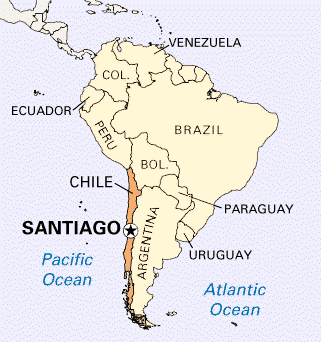
\includegraphics[width=\linewidth]{santiago-map.png}
      \end{wrapfigure}
\normalsize{
          \item 1,645 infants began SLCS between 1991-1996
          \item \raggedright Current sample recruited from 2 of 3 randomized control trial groups (n=888)
          \item  n=677 with infancy and adolescent data and of those n=546 with genotyped data (platform: Multi-Ethnic Global Array (MEGA))
          \item Low to middle income status in Chile.
          \item Ancestrally mixed American Indian and Spanish descent families
          \item Lipid traits measured after overnight fasting at mean age 17 years.
          }
    }
  \end{itemize}

  \end{block}

  \end{beamercolorbox}
  \end{column}
    % ---------------------------------------------------------%
    % end the 1st column
    % ---------------------------------------------------------%

% ---------------------------------------------------------%
% Set up 2nd column
% ---------------------------------------------------------%

\begin{column}{\twocolwid}
\begin{beamercolorbox}[center,wd=\textwidth]{postercolumn}

        % -----------------------------------------------------------
        % 2-1
        % -----------------------------------------------------------
        \begin{block}{Methods}
        
        \begin{enumerate}[1.]
          \item Test additive association between lipid traits and adequately powered single risk variants.
            \begin{itemize} \normalsize
              \item 76 common lipid variants selected from a European genome-wide meta-analysis with strongest independent signal.
              \item Association tests include 6 single variants with \textit{a priori} power > 0.80.
            \end{itemize}
          \item Assess the association of weighted genetic risk scores (wGRS) on lipid traits using linear regression model.
       \begin{itemize} \normalsize
           \item Coefficients for wGRS and power calculations based on European adult association studies.
              \end{itemize}
          \item Characterize proportion of variance explained by lipid variants.
          \end{enumerate}
% \vskip0.5em
% \toprule[2mm]
% \vskip0.5em

        \end{block}
        \vskip1ex

        % -----------------------------------------------------------
        % 2-2
        % -----------------------------------------------------------
        \begin{block}{Results}
        
        % Point to code to make all tables from summary statistics run on Kure
        % These figures were originally made for Dec 2016 presentation
        





\centering\normalsize Table. Sample descriptive statistics
\resizebox{\linewidth}{!}{%
\begin{normalsize}
\color{black}
\begin{tabular}{lcllcllc}
\hline
\multicolumn{1}{c}{\textbf{}}&&\multicolumn{2}{c}{\textbf{Chile}}&&\multicolumn{2}{c}{\textbf{Finland}}\\ 
\cline{3-4}\cline{6-7}
\textbf{Measure}&&\textbf{n=263}&\textbf{n=283}&&\textbf{n=661}&\textbf{n=555}\\ 
\hline
log(TG (mmol/l))&&1.44 (0.53)&1.38 (0.6)&&0.900 (0.37)&0.911 (0.39)\\ 
LDL-C (mmol/l)&&5.26 (1.55)&5.02 (1.53)&&3.07 (0.79)&2.91 (0.79)\\ 
HDL-C (mmol/l)&&2.3 (0.77)&2.05 (0.66)&&1.55 (0.29)&1.34 (0.24)\\ 
TC (mmol/l)&&8.55 (1.79)&7.96 (1.65)&&5.02 (0.89)&4.67 (0.84)\\ 
Age (years)&&16.77 (0.3)&16.76 (0.31)&&18&18\\ 
BMI (kg/m2)&&23.25 (5.33)&22.31 (5.12)&&--&--\\ 
HDL wGRS&&33.13 (3.47)&33.20 (3.42)&&32.46 (3.36)&32.62 (3.41)\\ 
LDL wGRS&&39.96 (6.38)&39.81 (6.40)&&42.1 (6.60)&41.9 (6.90)\\ 
TG wGRS&&138.84 (17.33)&138.32 (17.40)&&132.71 (16.81)&131.91 (15.72)\\ 
\hline
\end{tabular}
\end{normalsize}
\color{black}

        }
        
        % First figure
        % %%%%%%%%%%%%%%%%%%%%%%%%%%%%%%%%%%%%%%%%%%%%%%%%%%


        % Run code chunk from tables-slides.R to make table from summary statistics run on Kure


        


\vskip0.75em

Figure 1. Association tests by variant and sample
% NOTE: these were determined via power calculations at ~\Documents\dissertation\unc-dissertation-markdown\includes\scripts\power-calcs-ind-assoc.Rmd
        \centering
        \begin{figure}
%        \caption{Candidate single variant tests of association by variant and sample}


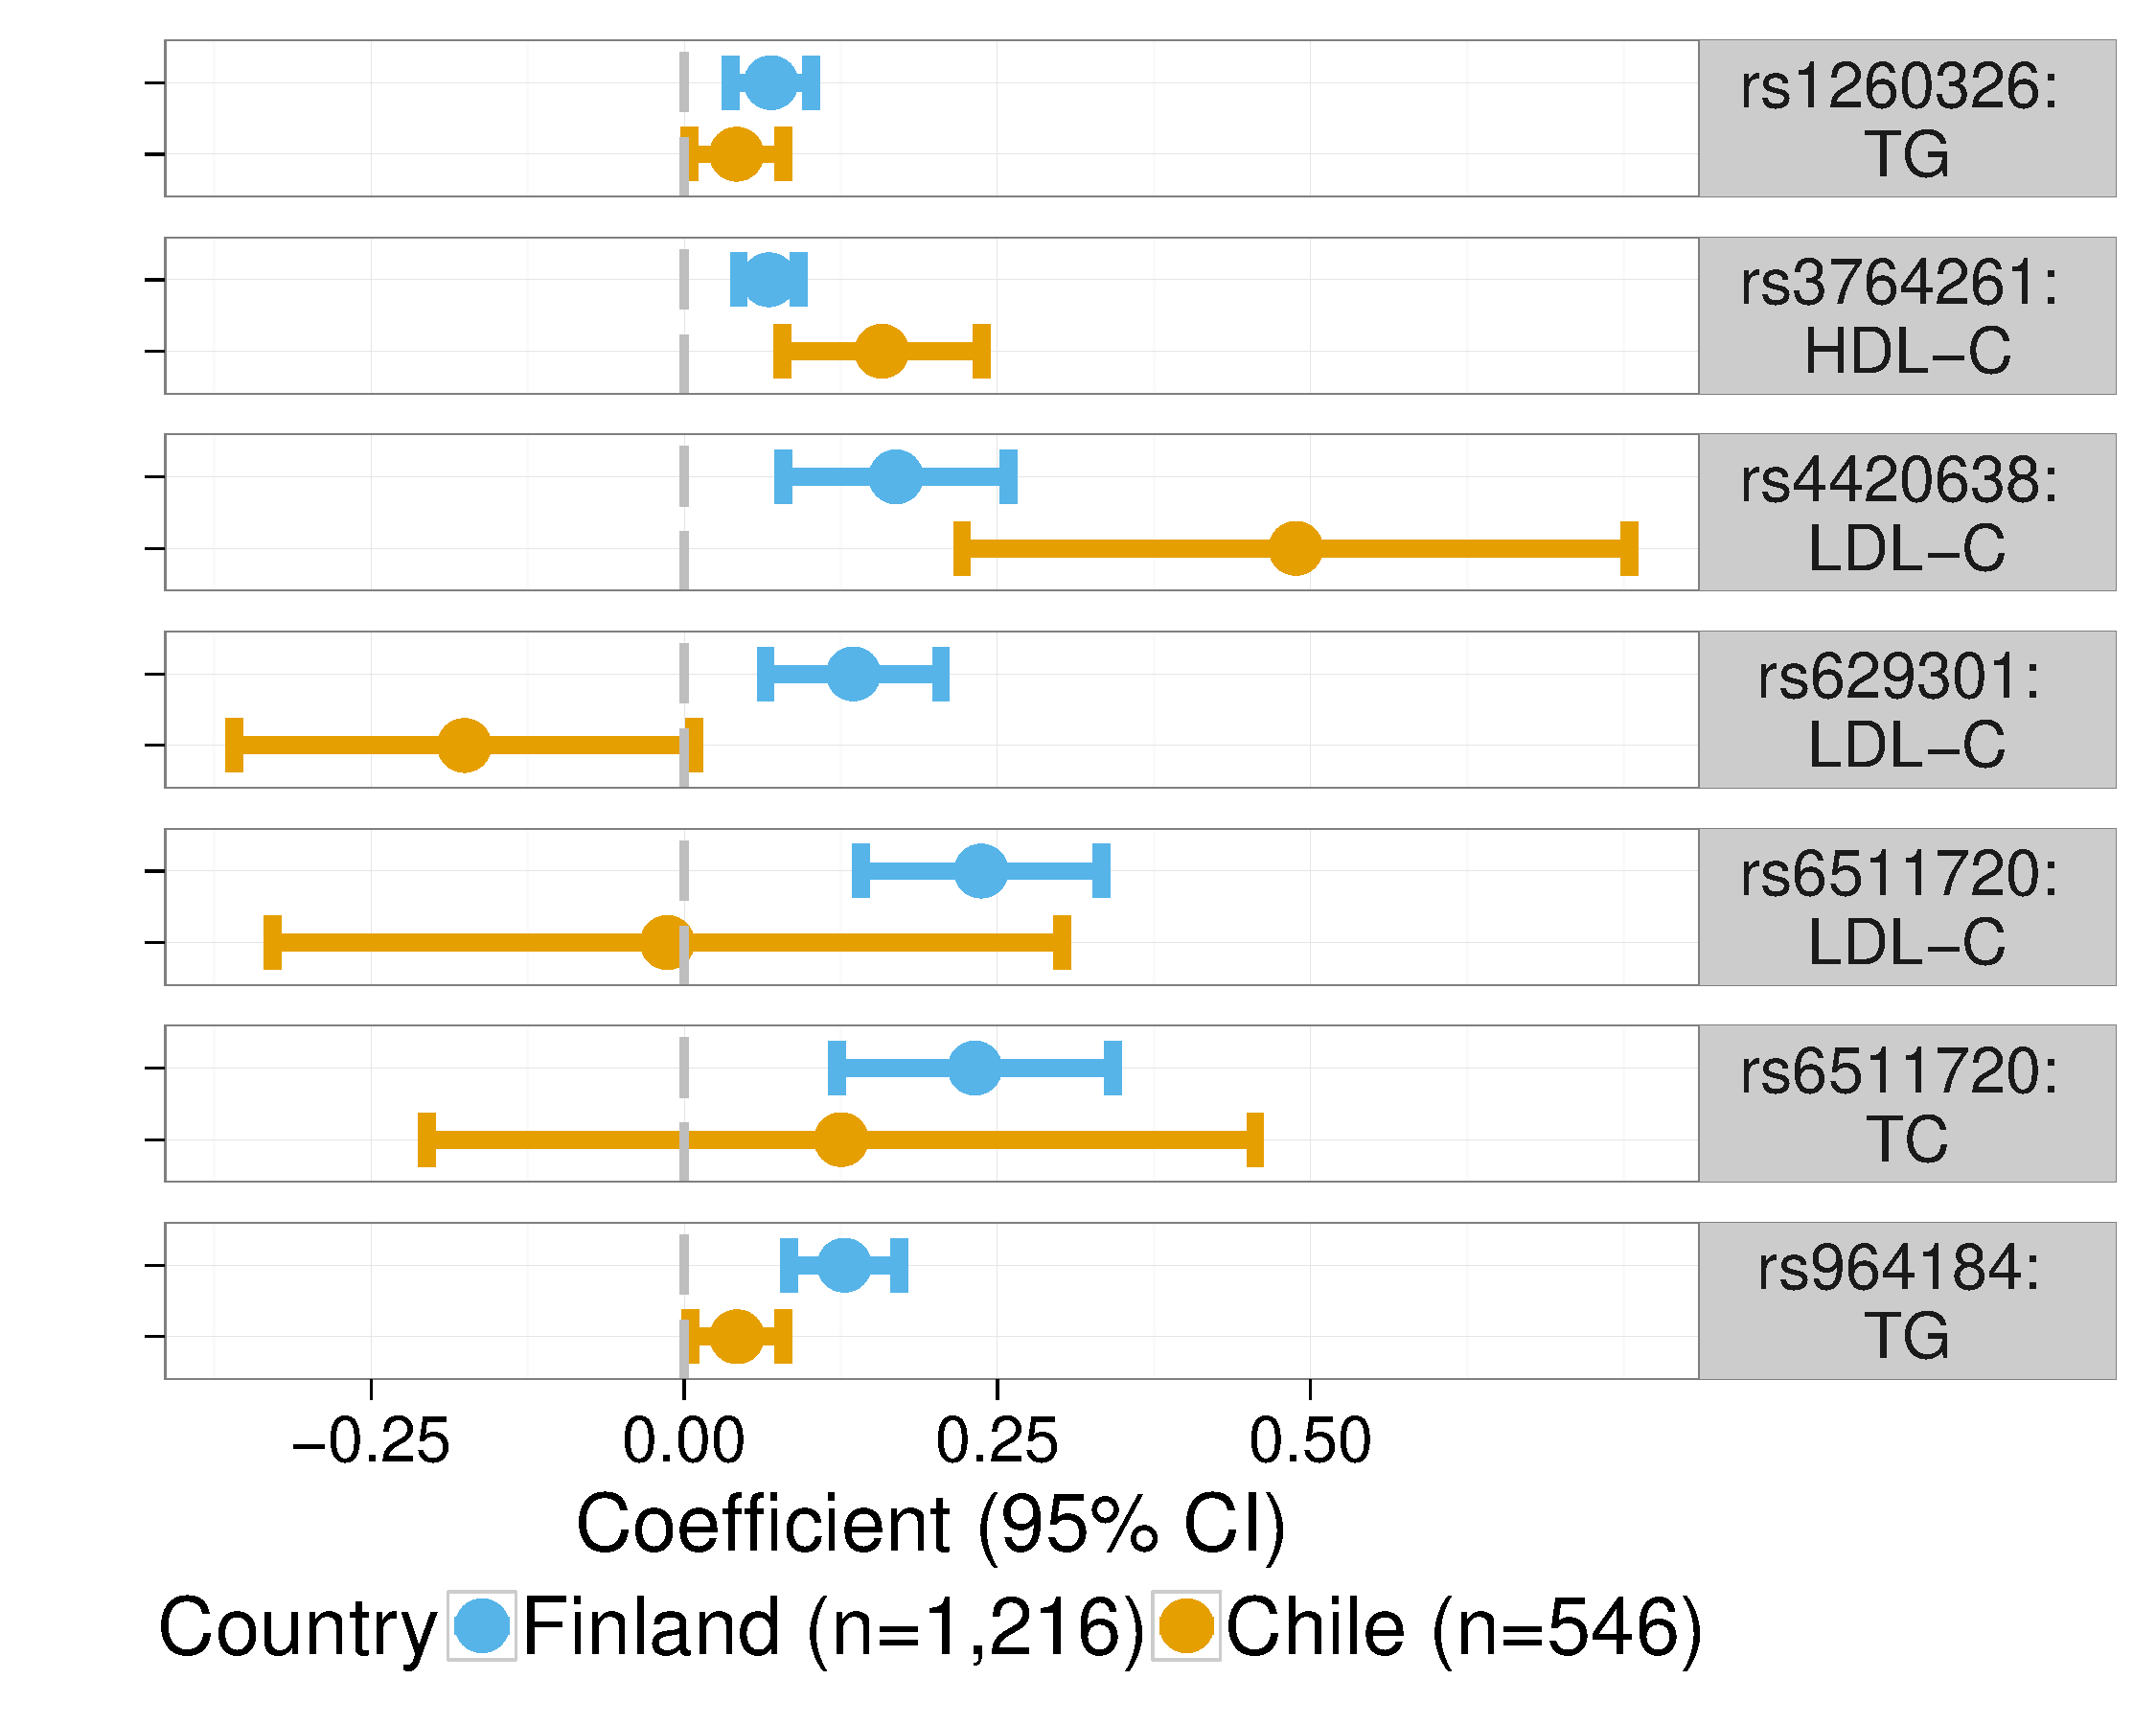
\includegraphics[width=\maxwidth]{figure/fig-assoc-2-poster-1} 

        \end{figure}
        
            \begin{itemize}\large
            \item \raggedright Four of the seven association tests were nominally statistically significant.
              \end{itemize}



        \end{block}

\end{beamercolorbox}
\end{column}

% ---------------------------------------------------------%
% end the 2nd column


% ---------------------------------------------------------%
% Set up 3rd column
% ---------------------------------------------------------%

\begin{column}{\threecolwid}
\begin{beamercolorbox}[center,wd=\textwidth]{postercolumn}


        \vfill

        % -----------------------------------------------------------
        % 3-1
        % -----------------------------------------------------------
        \begin{block}{Results, cont...}
        
        
          
        % Second figure
        % %%%%%%%%%%%%%%%%%%%%%%%%%%%%%%%%%%%%%%%%%%%%%%%%%%
        \centering
\normalsize{Figure 2. wGRS regression coefficients by sample and sex}

% Run code chunk from tables-slides.R to make table from summary statistics run on Kure



        \begin{figure}
\begin{knitrout}
\definecolor{shadecolor}{rgb}{0.969, 0.969, 0.969}\color{fgcolor}
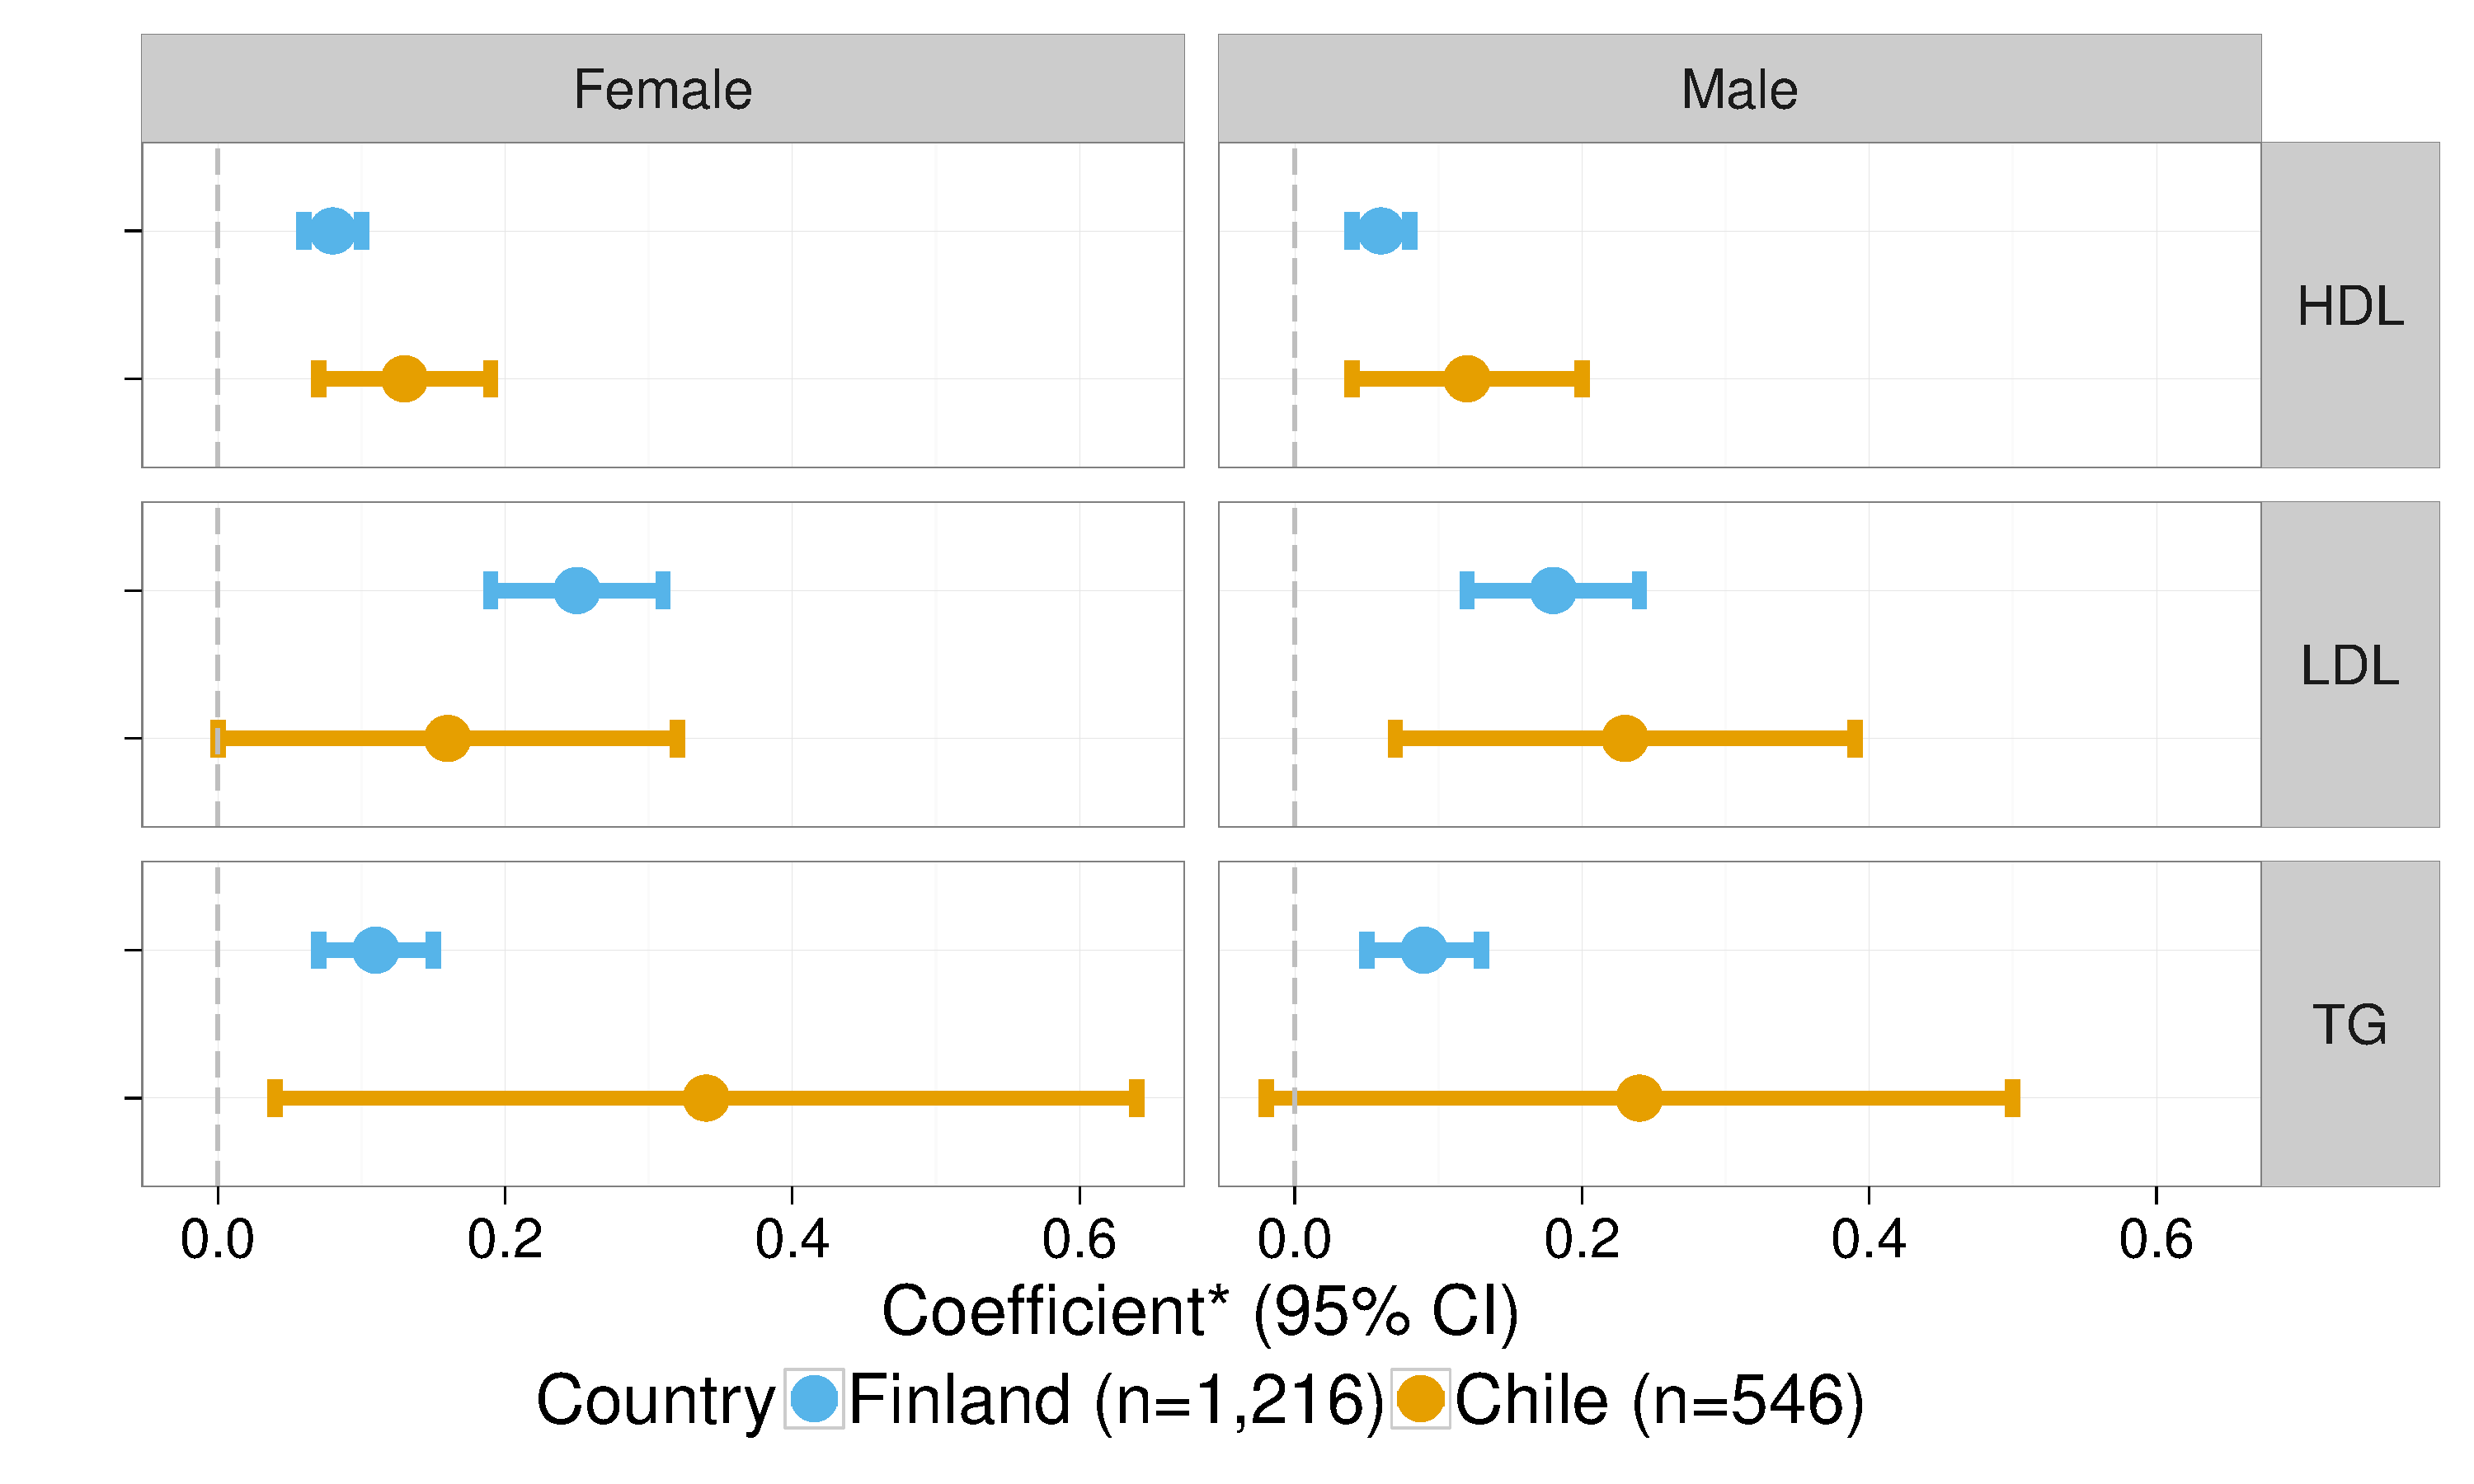
\includegraphics[width=\maxwidth]{figure/fig3-2-poster-1} 

\end{knitrout}
        \end{figure}
        
        
\vspace{-0.4em}
        
        \begin{addmargin}[2cm]{0cm}
        \begin{flusChileaneft}
        \footnotesize{*Coefficients represent change in outcome per 1 SD change in wGRS, adjusted for first five principal components representing ancestry.}
        \end{flusChileaneft}
        \end{addmargin}
        
        \begin{itemize}\large
            \item \raggedright  wGRS has stronger association for each lipid outcome in Chilean versus Finnish sample except LDL-C for females.
            \end{itemize}
\vskip0.5em

        % Third figure
        % %%%%%%%%%%%%%%%%%%%%%%%%%%%%%%%%%%%%%%%%%%%%%%%%%%

% Run code chunk from tables-slides.R to make table from summary statistics run on Kure


        

\normalsize{Figure 3. Proportion of variance explained by genetic variants, by sex}
        \centering
        \begin{figure}

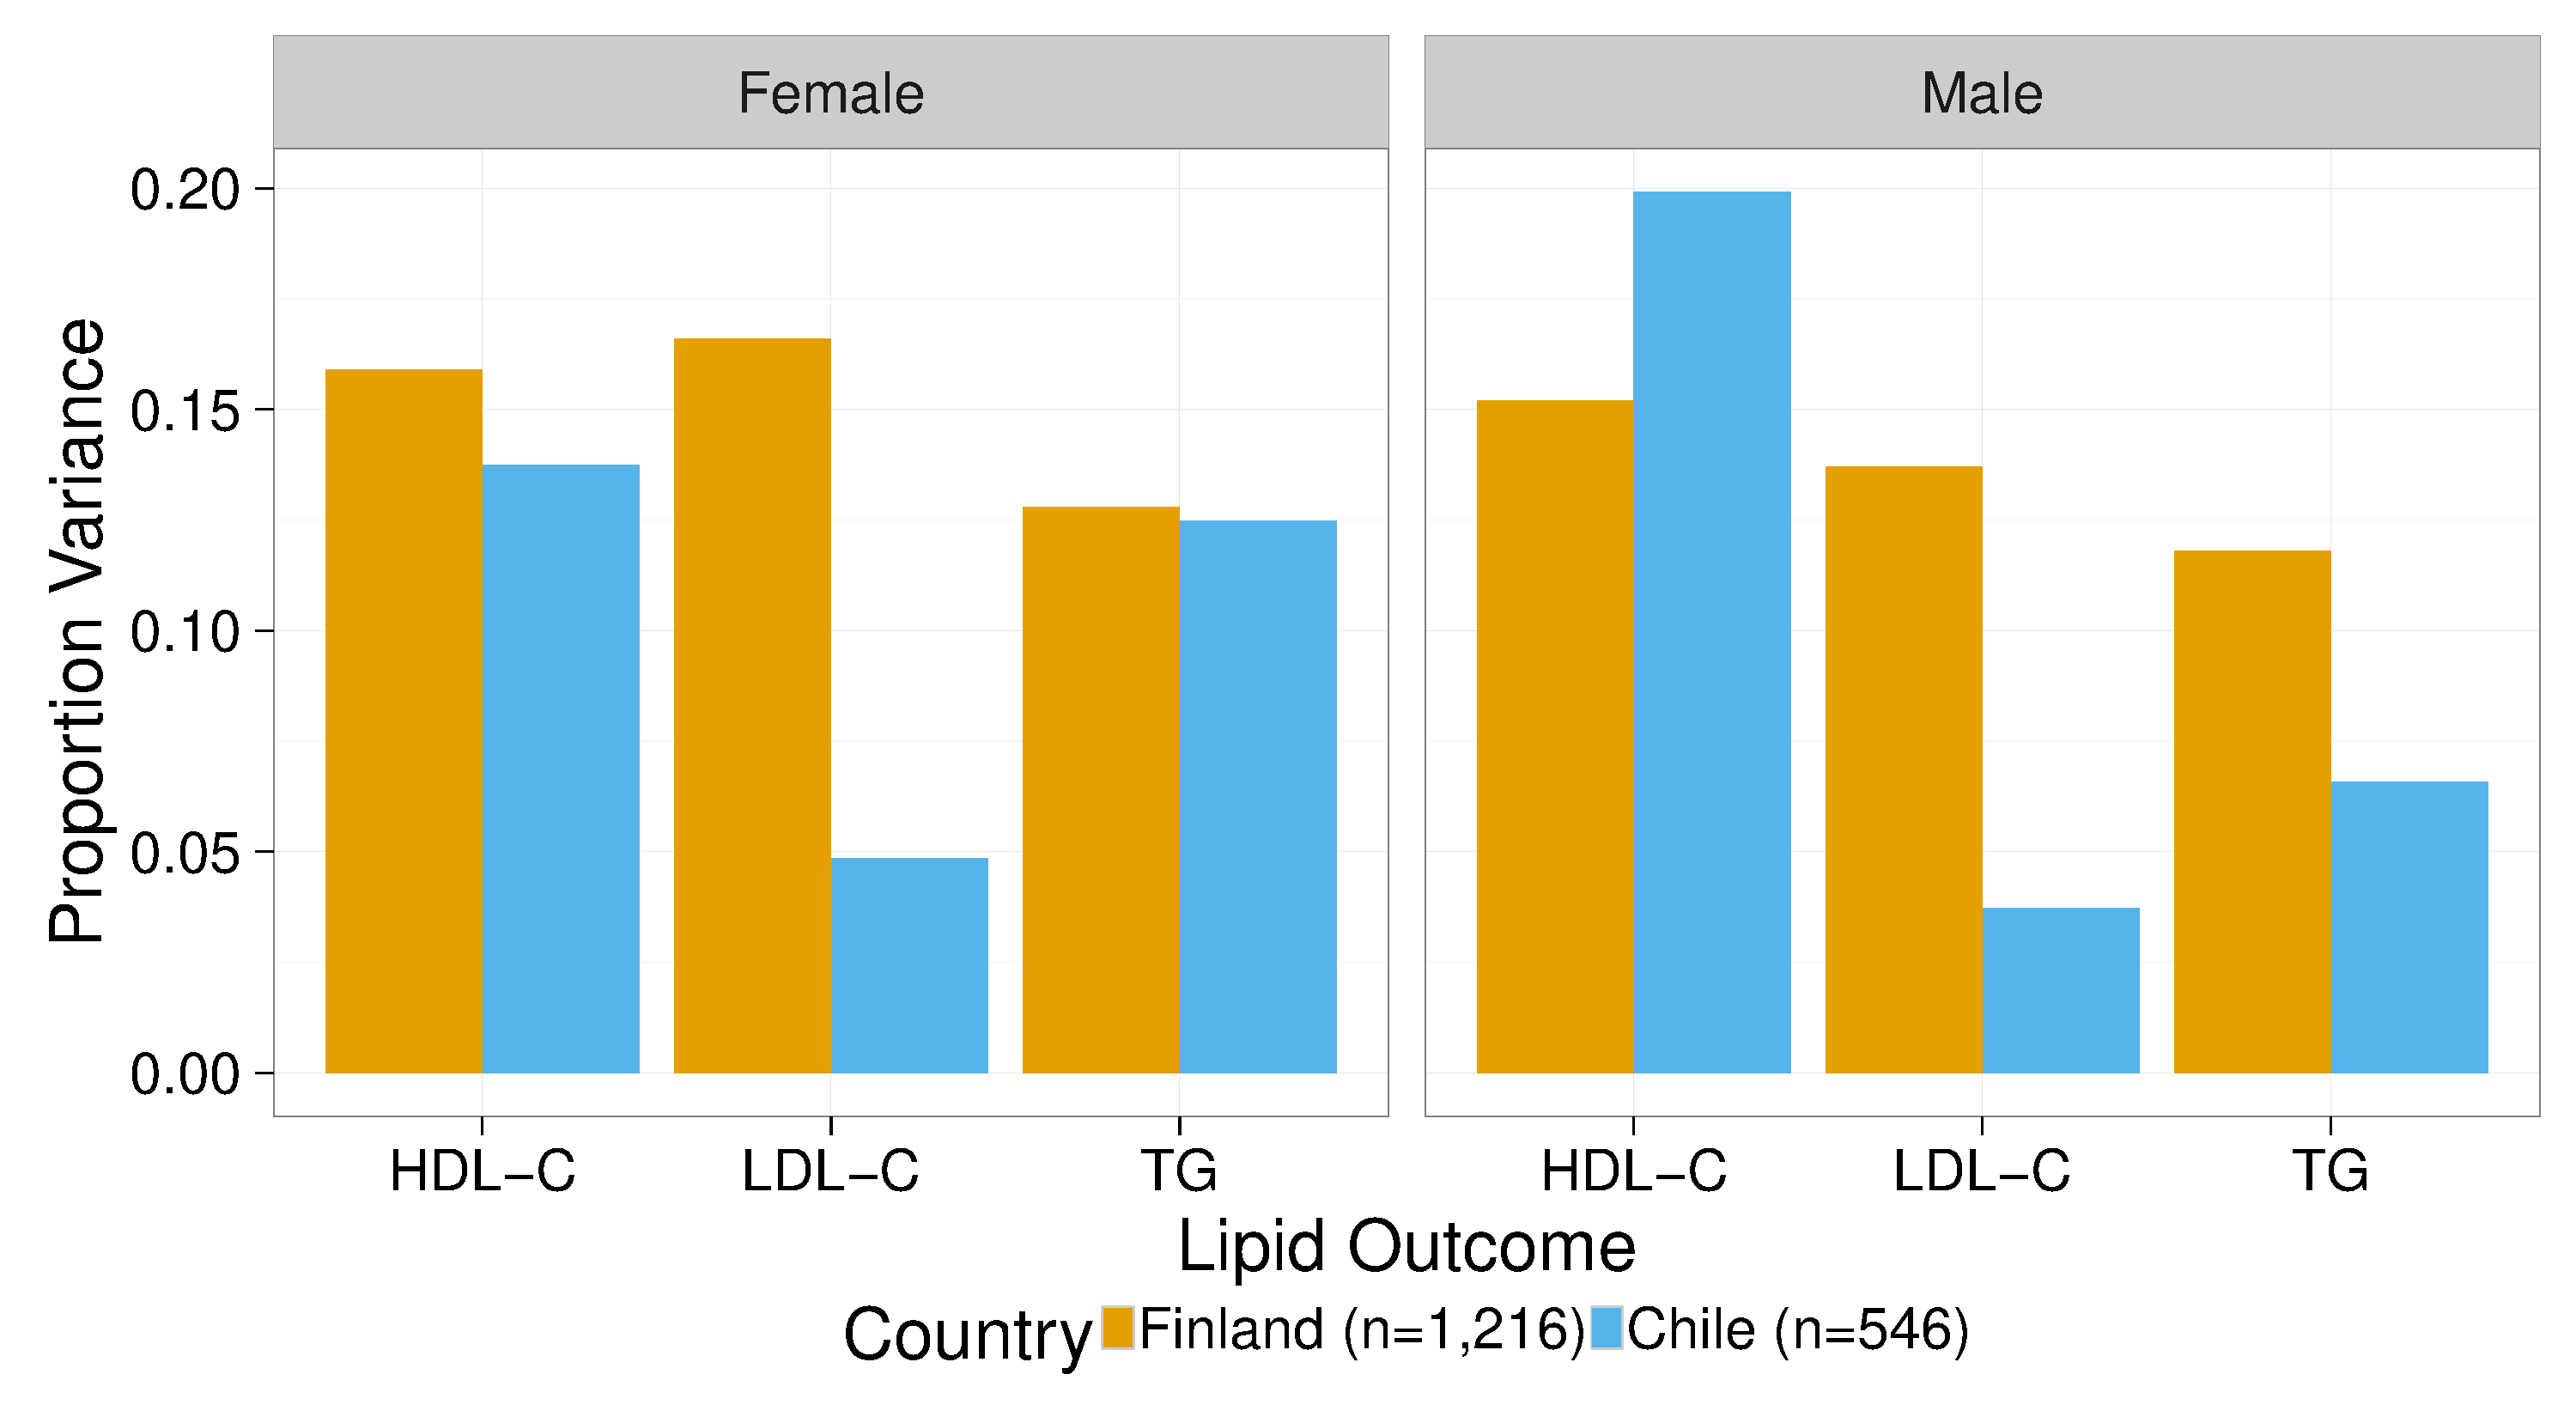
\includegraphics[width=\maxwidth]{figure/fig2-2poster-1} 

        \end{figure}

%        \begin{mdframed}[style=MyFrame]
          \begin{itemize}\large
            \item \raggedright LDL-C-related variants explain much less variance in Chilean sample.
            \end{itemize}
%            \end{mdframed}
        
        \end{block}
        
        \vskip1ex
        \vfill
        
        % -----------------------------------------------------------
        % 3-2
        % -----------------------------------------------------------
        \begin{block}{Summary}
        
          \begin{itemize}
            \item Significant associations support concordance of effects across European and HL populations first found in adults for these loci.
            \item Genetic risk evident in childhood presents across different populations, emphasizing younger ages as a point for intervention.
            \end{itemize}
        \end{block}
        
        \vskip1ex
        \vfill


        % -----------------------------------------------------------
        % 3-3
        % -----------------------------------------------------------
        % \begin{block}{References}
        %   %\scriptsize{%          \printbibliography{}}
        %   \scriptsize
        %   (1) \fullcite{coram_genome-wide_2013} \\
        %   (2) \fullcite{lozoff_behavioral_2003} \\
        %   (3) \fullcite{tikkanen_association_2011} \\
        %   (4) \fullcite{teslovich_biological_2010} \\
        %   (5) \fullcite{buscot_combined_2016} \\
        %   % see https://en.wikibooks.org/wiki/LaTeX/Fonts
        % \end{block}

\end{beamercolorbox}
\end{column}
% ---------------------------------------------------------%
% end the 3rd column
% ---------------------------------------------------------%

\end{columns}

\end{frame}
\end{document}
